\documentclass[stu,12pt,floatsintext]{apa7}

\usepackage[american]{babel}
\usepackage{csquotes}
\usepackage{graphicx}
\usepackage{booktabs}
\usepackage{float}
\usepackage{hanging}

\title{Seeing the Gap: An Interactive Shopping-Platform Simulation for High School Students}
\shorttitle{Seeing the Gap}
\authorsnames{Zhiyan Zhang}
\authorsaffiliations{Shanghai Pinghe School}
\course{AI for Social Sciences}
\professor{Research Advisor: Lawted Wu}
\duedate{July 2026}

\abstract{High school students routinely encounter discounts, recommendations, countdowns, reviews, and default options, yet confidence in consumer judgment may not correspond to behavior within these interfaces. Existing research has examined advertising literacy, self-report bias, consumer decision styles, and manipulative interface design, but these strands have rarely been combined in a short interactive experience that compares self-perception with simulated choice. This study developed a browser-based shopping-platform simulation in which users completed pre-use measures, made five controlled shopping decisions, received a rule-based comparison of their responses and actions, and completed the same awareness measure afterward. Using a within-participant pre-test/post-test design, the study examined 41 completed anonymous sessions. The mean awareness score decreased from 3.821 before the simulation to 3.228 after it, with a mean change of -0.593. Thirty participants gave a lower post-test score, five stayed the same, and six increased. This pattern is interpreted as self-perception recalibration: after seeing their simulated choices, many participants appeared less confident that they could predict or explain their own consumer behavior. Rule-based mismatch indicators also supported this interpretation. Thirty-one of the 41 participants had at least one mismatch between self-perception and simulated choice, and participants with more mismatches showed larger decreases in post-test self-rating.}
\keywords{consumer self-perception, high school students, shopping platform, self-report bias, interface design}

\begin{document}
\maketitle

\section{Introduction}

High school students make consumer decisions within a dense digital environment shaped by shopping platforms, short videos, product recommendations, peer culture, online reviews, discounts, membership systems, and interface design. These decisions involve more than personal preference or available money. Urgency messages, default options, price framing, and conflicting information can shape behavior at the point of choice.

Many students also hold an image of themselves as careful, budget-conscious, or information-aware consumers. Consumer socialization research frames this self-image as something young people develop through family, media, platforms, and market experiences (John, 1999). Persuasion knowledge research also shows that consumers learn to recognize marketers' motives and tactics, but that knowledge still has to be activated in concrete situations (Friestad \& Wright, 1994). Therefore, self-perception does not necessarily indicate how students will act in a realistic choice environment. Advertising knowledge may not be activated at the moment of exposure (Rozendaal et al., 2011), and self-report measures may reflect socially desirable or idealized descriptions rather than observed behavior (Donaldson \& Grant-Vallone, 2002). Research on verbal reports also warns that people may not have direct access to the mental processes behind their own choices (Nisbett \& Wilson, 1977). This distinction makes it necessary to compare stated judgment habits with actions rather than rely on self-report alone.

Research on adolescents' self-reported advertising literacy shows that young people can describe their ability to recognize, understand, and resist advertising (De Jans et al., 2018). Consumer decision-making research likewise treats judgment as multidimensional, including price awareness, impulsiveness, quality concern, and confusion from excessive choice (Sproles \& Kendall, 1986). At the interface level, online shopping environments have used urgency, social proof, default choices, and hidden costs to guide behavior (Mathur et al., 2019). Controlled vignette methods offer a way to retain recognizable situations while isolating specific mechanisms for analysis (Atzmüller \& Steiner, 2010; Steiner et al., 2017).

The present study connects these areas in one interactive artifact. Rather than classifying participants as rational or irrational, it examines whether a shopping-platform simulation can make differences between consumer self-perception and simulated choice more visible. The research question is: How did an interactive shopping-platform simulation affect high school students' recognition of gaps between their consumer self-perception and their simulated shopping choices? It was hypothesized that the simulation would make this gap more visible to participants. In the original plan, this was expected to appear as a higher post-test awareness score. In the final analysis, the score direction was interpreted through the wording of the repeated items: if participants gave lower post-test ratings of their ability to predict or explain their own choices, this could indicate that they had recognized their earlier self-confidence was too high.

This framing matters for a social-science project because the goal is not to judge whether a student made a ``good'' or ``bad'' purchase. The more important question is how students understand themselves inside a designed consumer environment. A student might say that reviews matter, but still submit an order quickly when a page creates urgency. Another student might say that add-on services do not influence them, but still keep a preselected paid option at checkout. These cases are not simply personal failures. They show how self-understanding, interface design, and moment-by-moment decision conditions interact.

\section{Methods}

\subsection{Artifact and Procedure}

The deployed artifact was a single-page, browser-based shopping-platform simulation designed for high school students. On entering the tool, participants answered two background questions concerning their monthly disposable-money range and product categories encountered during the previous 30 days. They then completed three pre-use awareness items and four consumer self-perception items. All seven items used five-point response scales. The self-perception items addressed budget impact, information checking, attention to additional services, and responses to sudden price reductions.

Participants subsequently completed five controlled shopping stages: a product feed, a price-drop pop-up, a product-detail page, a checkout page containing a preselected paid service, and a final page combining conflicting review information with a budget warning. Each stage recorded one selected action. A short addition task separated consecutive shopping stages and was not included in the consumer measures. No real purchase or payment occurred.

The product feed displayed four cards. Product categories were selected from the participant's recent-category responses and from categories that the participant had not selected. Displayed prices were calculated deterministically from the budget anchor assigned to the selected disposable-money range, using target ratios of 8\%, 12\%, 18\%, and 32\%. This design kept the simulation close to an everyday shopping interface while still allowing the project to compare users under the same basic structure. The simulation avoided asking users to write a long explanation during the main shopping stages, because that could make the research purpose too obvious and change how they acted.

The system recorded a randomly generated session identifier, background and scale responses, action order, stage, selected action, product category and name, whether the product belonged to a recently encountered category, displayed price, price as a percentage of the budget anchor, and decision-time fields from the webpage flow. These records allowed the analysis to connect three layers of data: what the participant said about themselves before the shopping task, what they clicked during the task, and how they rated their self-understanding after seeing the result page.

After the fifth stage, the result screen displayed rule-based comparisons between self-perception and recorded choices. It then administered the same three awareness items as a post-test, a five-point rating of perceived profile fit, and two optional open-text prompts asking what the participant had learned and which page elements had influenced the choices.

All product names, shopping messages, reviews, page mechanisms, and result-classification rules were prewritten and curated for the study. The artifact did not call an AI model, a generative-AI service, a live shopping service, or a prediction API. Its personalized product feed and ``consumer profile'' were deterministic mock outputs derived from the participant's budget range, selected categories, scale responses, and recorded actions. Supabase REST endpoints were used only to store anonymous research records.

The shopping mechanisms were selected because they appear often in ordinary online consumer environments and because each could be tied to a specific self-perception statement. The price-drop prompt tested whether users who described themselves as resistant to sudden discounts would still follow a time-sensitive cue. The detail page tested whether users who said they checked information would inspect reviews or rules before moving forward. The checkout page tested attention to default paid services. The final review page tested whether budget pressure and conflicting information changed the decision path.

\subsection{Research Design and Measures}

The study used a single-group, within-participant pre-test/post-test design. The independent variable was measurement time relative to the simulation: pre-use versus post-use. The primary dependent variable was awareness of the gap between intended and simulated shopping behavior, operationalized as the mean of three repeated items: perceived ability to predict one's shopping choices, perceived correspondence between intentions and actions, and perceived ability to identify influential page information. The original exploratory success criterion expected post-use awareness to increase. During analysis, the direction of the score was interpreted more carefully: a lower post-test self-rating may also indicate that participants became less overconfident after seeing the gap between their self-image and their choices. Therefore, the main interpretation focuses on self-perception recalibration rather than confidence increase alone.

Secondary behavioral outcomes included product-path selection, responses to the price-drop prompt, review or rule checking, retention or cancellation of the default paid service, continuation under budget pressure, selection of a cheaper specification, stopping the simulated purchase, action order, and decision-time measures. The interface also generated descriptive mismatch indicators by comparing each self-perception dimension with its corresponding recorded action.

The four mismatch indicators were exploratory and rule-based. A budget-control gap was marked when a participant reported strong budget sensitivity but still submitted the final simulated order under budget pressure. An information-checking gap was marked when a participant reported strong information-checking habits but did not choose review or rule-checking actions. A default-option gap was marked when a participant reported attention to details or extra services but kept the preselected paid service at checkout. A time-pressure gap was marked when a participant reported resistance to sudden price drops but followed a price-drop path or moved quickly toward purchase. These indicators were not treated as clinical or personality labels. They were used as descriptive tools for comparing self-perception and behavior within the simulation.

\subsection{Consent and Data Handling}

Informed consent was presented as a required first screen. It stated that participation was anonymous, voluntary, and limited to classroom research. It also stated that participants could leave at any time by closing the page, and that names, telephone numbers, student identifiers, real purchase records, and payment information would not be collected. Participants continued by selecting ``I agree, start the test''; those who did not agree were instructed to close the page. Records were linked through a randomly generated session identifier rather than a direct personal identifier.

The consent page was important because the artifact resembled a shopping platform, but the study did not involve real shopping. Participants needed to know that they were not making payments and that the data would be used only for the course project. The project also avoided collecting identifiable demographic details beyond broad school-level context, because the main analysis did not require names, accounts, phone numbers, or precise identities.

\subsection{Participants, Recruitment, and Analysis}

The target population consisted of high school students. Participants were recruited through the researcher's personal network from July 12 to July 22, 2026. The website link was shared with classmates, a class group chat, and the researcher's social media feed. Participation was voluntary, and no reward or compensation was offered. The analysis used 41 completed anonymous sessions recorded in the project database. A completed session was defined as one session with a pre-test awareness score, five recorded shopping-stage actions, and a post-test feedback record.

The analysis protocol treated each anonymous session as one case. Before calculating results, a valid case was defined as a completed anonymous session with one row in the session table, five shopping-stage event records, one result-feedback record, and non-missing pre-test and post-test awareness scores. This cleaning rule focused on completion quality. It did not remove records because their answers supported or contradicted the hypothesis.

Pre-test and post-test awareness scores and within-participant change scores were summarized using counts, means, standard deviations, and direction of change. Frequencies and percentages were calculated for recorded actions and rule-based mismatch indicators. A paired-samples t statistic was calculated as an exploratory test of within-participant change. Because this was a classroom prototype study with a small and non-random sample, inferential values are reported as supportive descriptive evidence rather than final proof.

The two open-text responses were treated as supplementary qualitative material. A simple theme-led coding approach was used for the first pass. Responses could receive more than one code because one sentence could mention several influences. The codes included time pressure or discount reminders, default service or checkout design, information checking or review conflict, budget or price concern, product interest, and self-perception recalibration. The qualitative coding was used to support the quantitative patterns, not to replace them.

\section{Results}

\subsection{Valid Sessions}

The final dataset contained 41 completed sessions. Each valid session had five recorded shopping-stage actions, so the action dataset contained 205 stage-level records. All 41 sessions had pre-test and post-test awareness scores.

\subsection{Pre-Test and Post-Test Awareness}

The mean pre-test awareness score was 3.821 (\textit{SD} = 0.628). The mean post-test awareness score was 3.228 (\textit{SD} = 0.529). The mean change score, calculated as post-test minus pre-test, was -0.593 (\textit{SD} = 0.673). Thirty participants had lower post-test scores, five participants had no change, and six participants had higher post-test scores.

An exploratory paired-samples calculation produced \textit{t}(40) = -5.646, with an approximate 95\% confidence interval for the mean change from -0.805 to -0.381. The standardized within-participant change was \textit{d}\textsubscript{z} = -0.882. The negative value means the post-test self-rating was lower than the pre-test self-rating on average.

\begin{figure}[H]
  \centering
  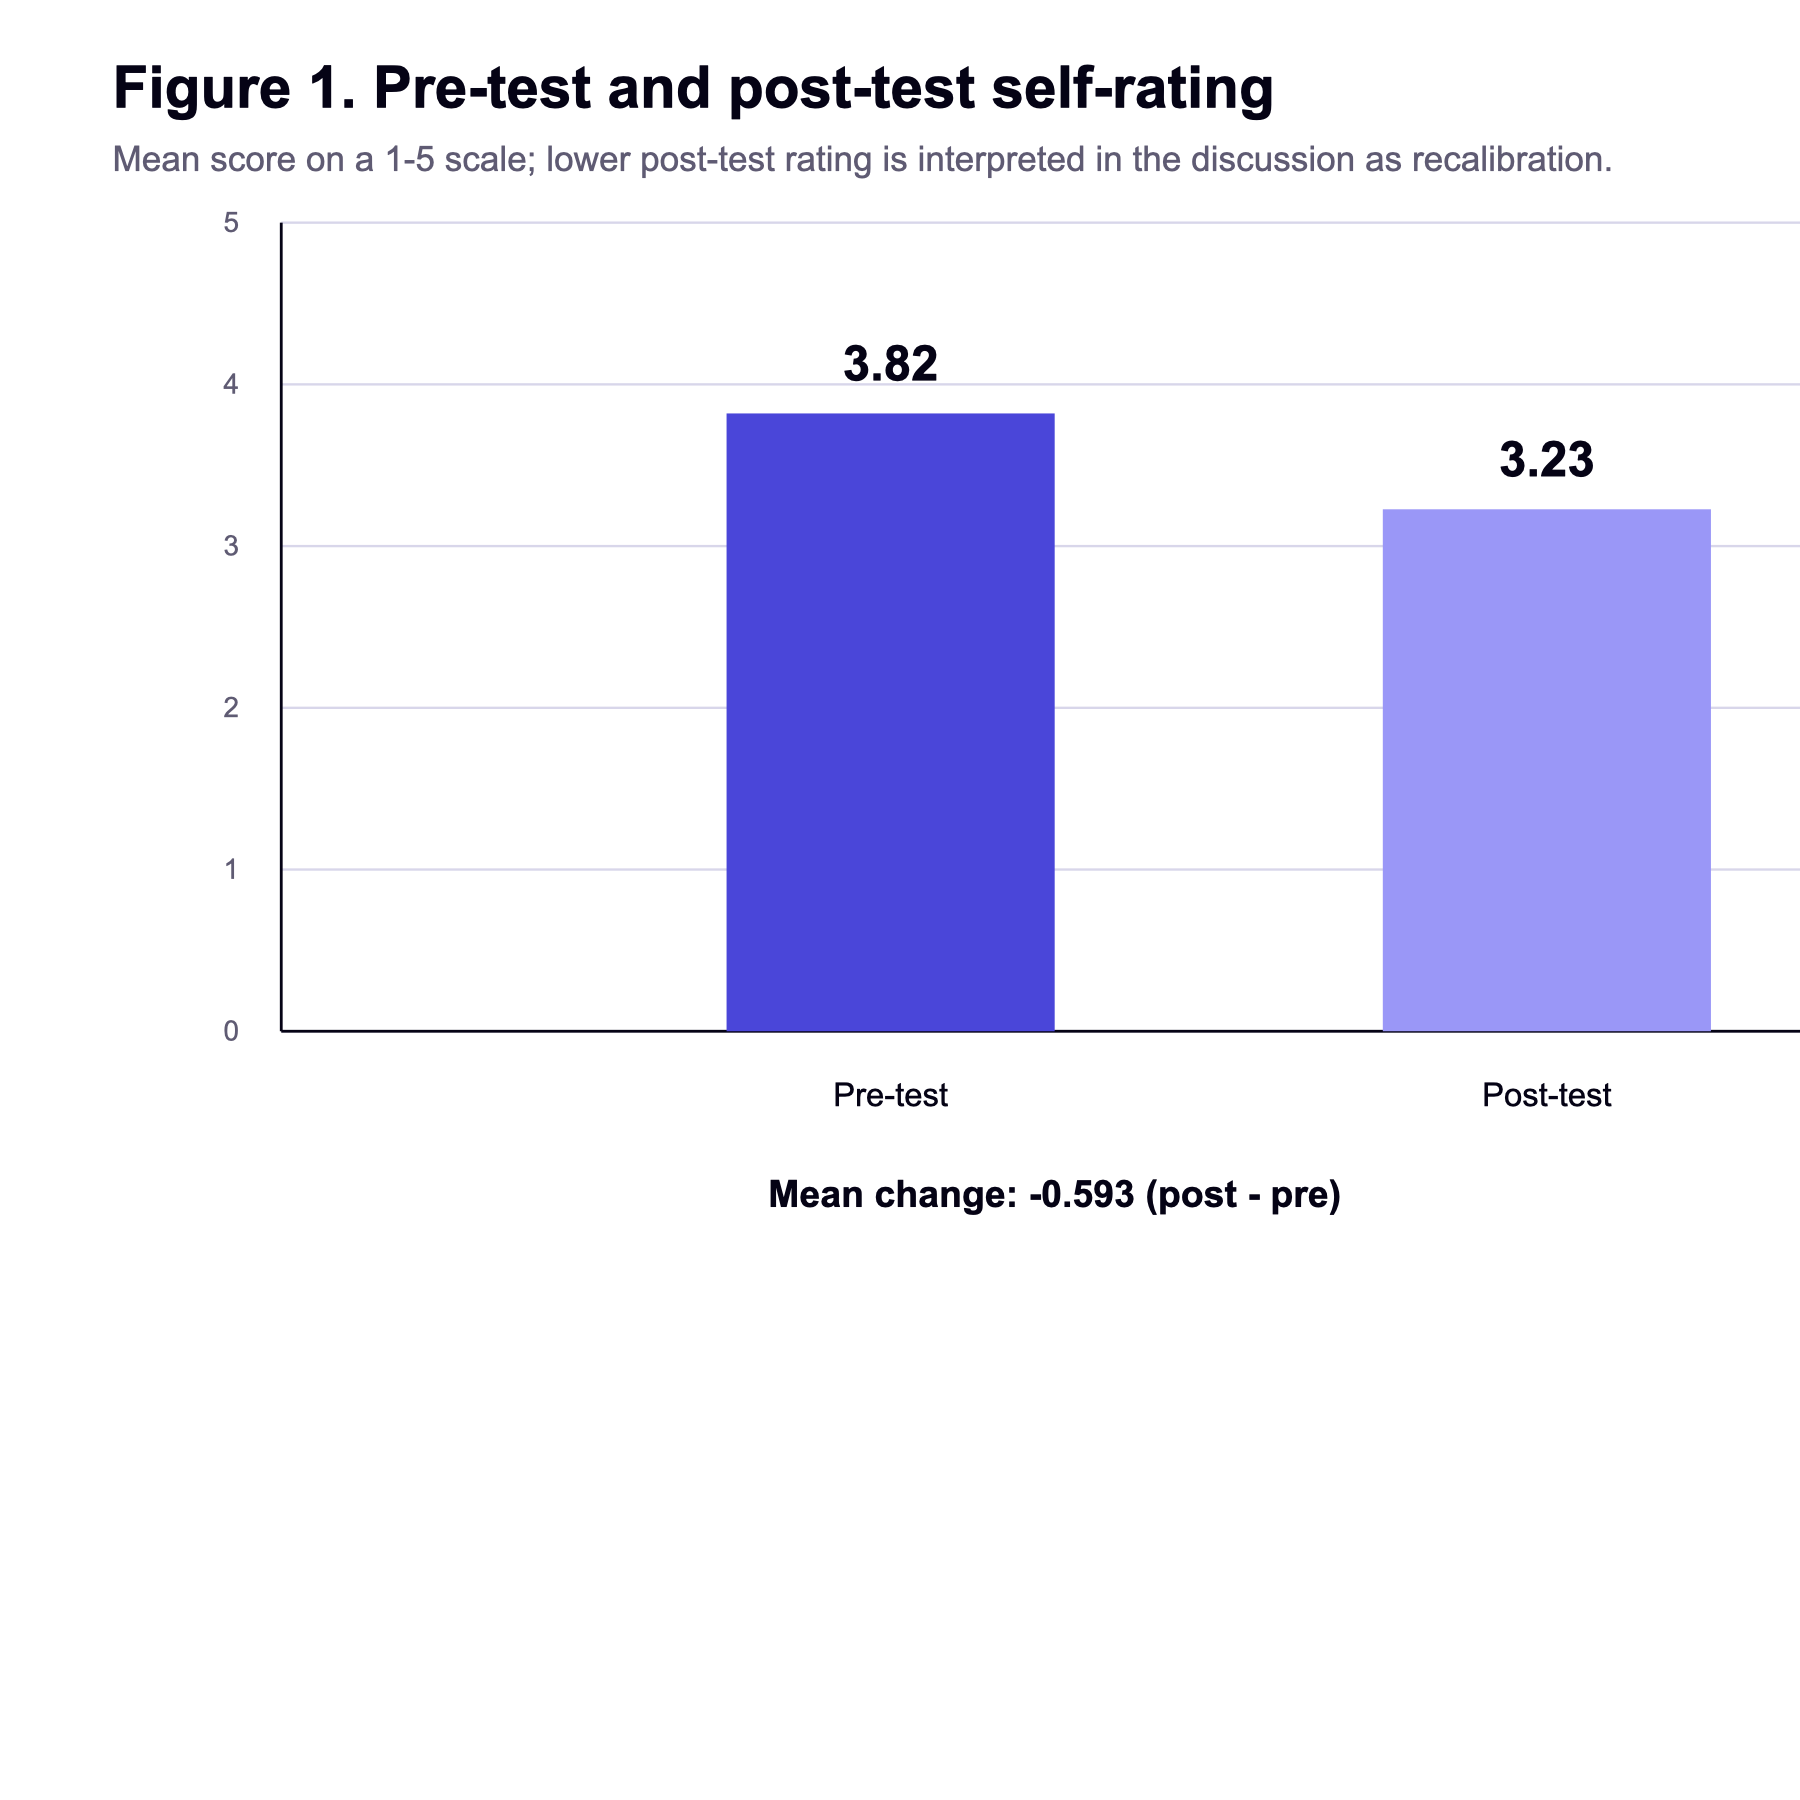
\includegraphics[width=.82\linewidth]{analysis/charts_png/pre-post-awareness.png}
  \caption{Pre-test and post-test self-rating.}
  \label{fig:prepost}
\end{figure}

\subsection{Simulated Shopping Choices}

All participants opened a product from the feed stage. In the price-drop pop-up stage, 21 participants viewed the price drop (51.2\%), 12 postponed the decision (29.3\%), and 8 closed the reminder (19.5\%). On the product-detail page, 15 chose immediate purchase (36.6\%), 9 added the product to cart (22.0\%), 11 checked reviews (26.8\%), and 6 checked rules (14.6\%).

The checkout stage showed the clearest default-option pattern. Twenty-seven participants kept the default paid service (65.9\%), while 8 cancelled it (19.5\%) and 6 checked more information (14.6\%). In the final review and budget-warning stage, 29 participants submitted the simulated order (70.7\%), 6 stopped (14.6\%), 4 checked more reviews (9.8\%), and 2 selected a cheaper option (4.9\%).

\subsection{Self-Perception and Choice Gaps}

Rule-based mismatch indicators compared each participant's self-perception answers with their recorded choices. Thirty-one participants, or 75.6\% of the sample, had at least one mismatch. The average mismatch count was 2.024 out of four possible gap dimensions.

The most common gaps were budget-control gap and default-option gap, each appearing in 22 participants (53.7\%). The information-checking gap appeared in 19 participants (46.3\%), and the time-pressure gap appeared in 20 participants (48.8\%).

Mismatch count was positively related to score recalibration. Participants with zero mismatch indicators had an average recalibration of 0.033 points, while participants with four mismatch indicators had an average recalibration of 1.277 points. The correlation between mismatch count and recalibration score was 0.758.

\begin{figure}[H]
  \centering
  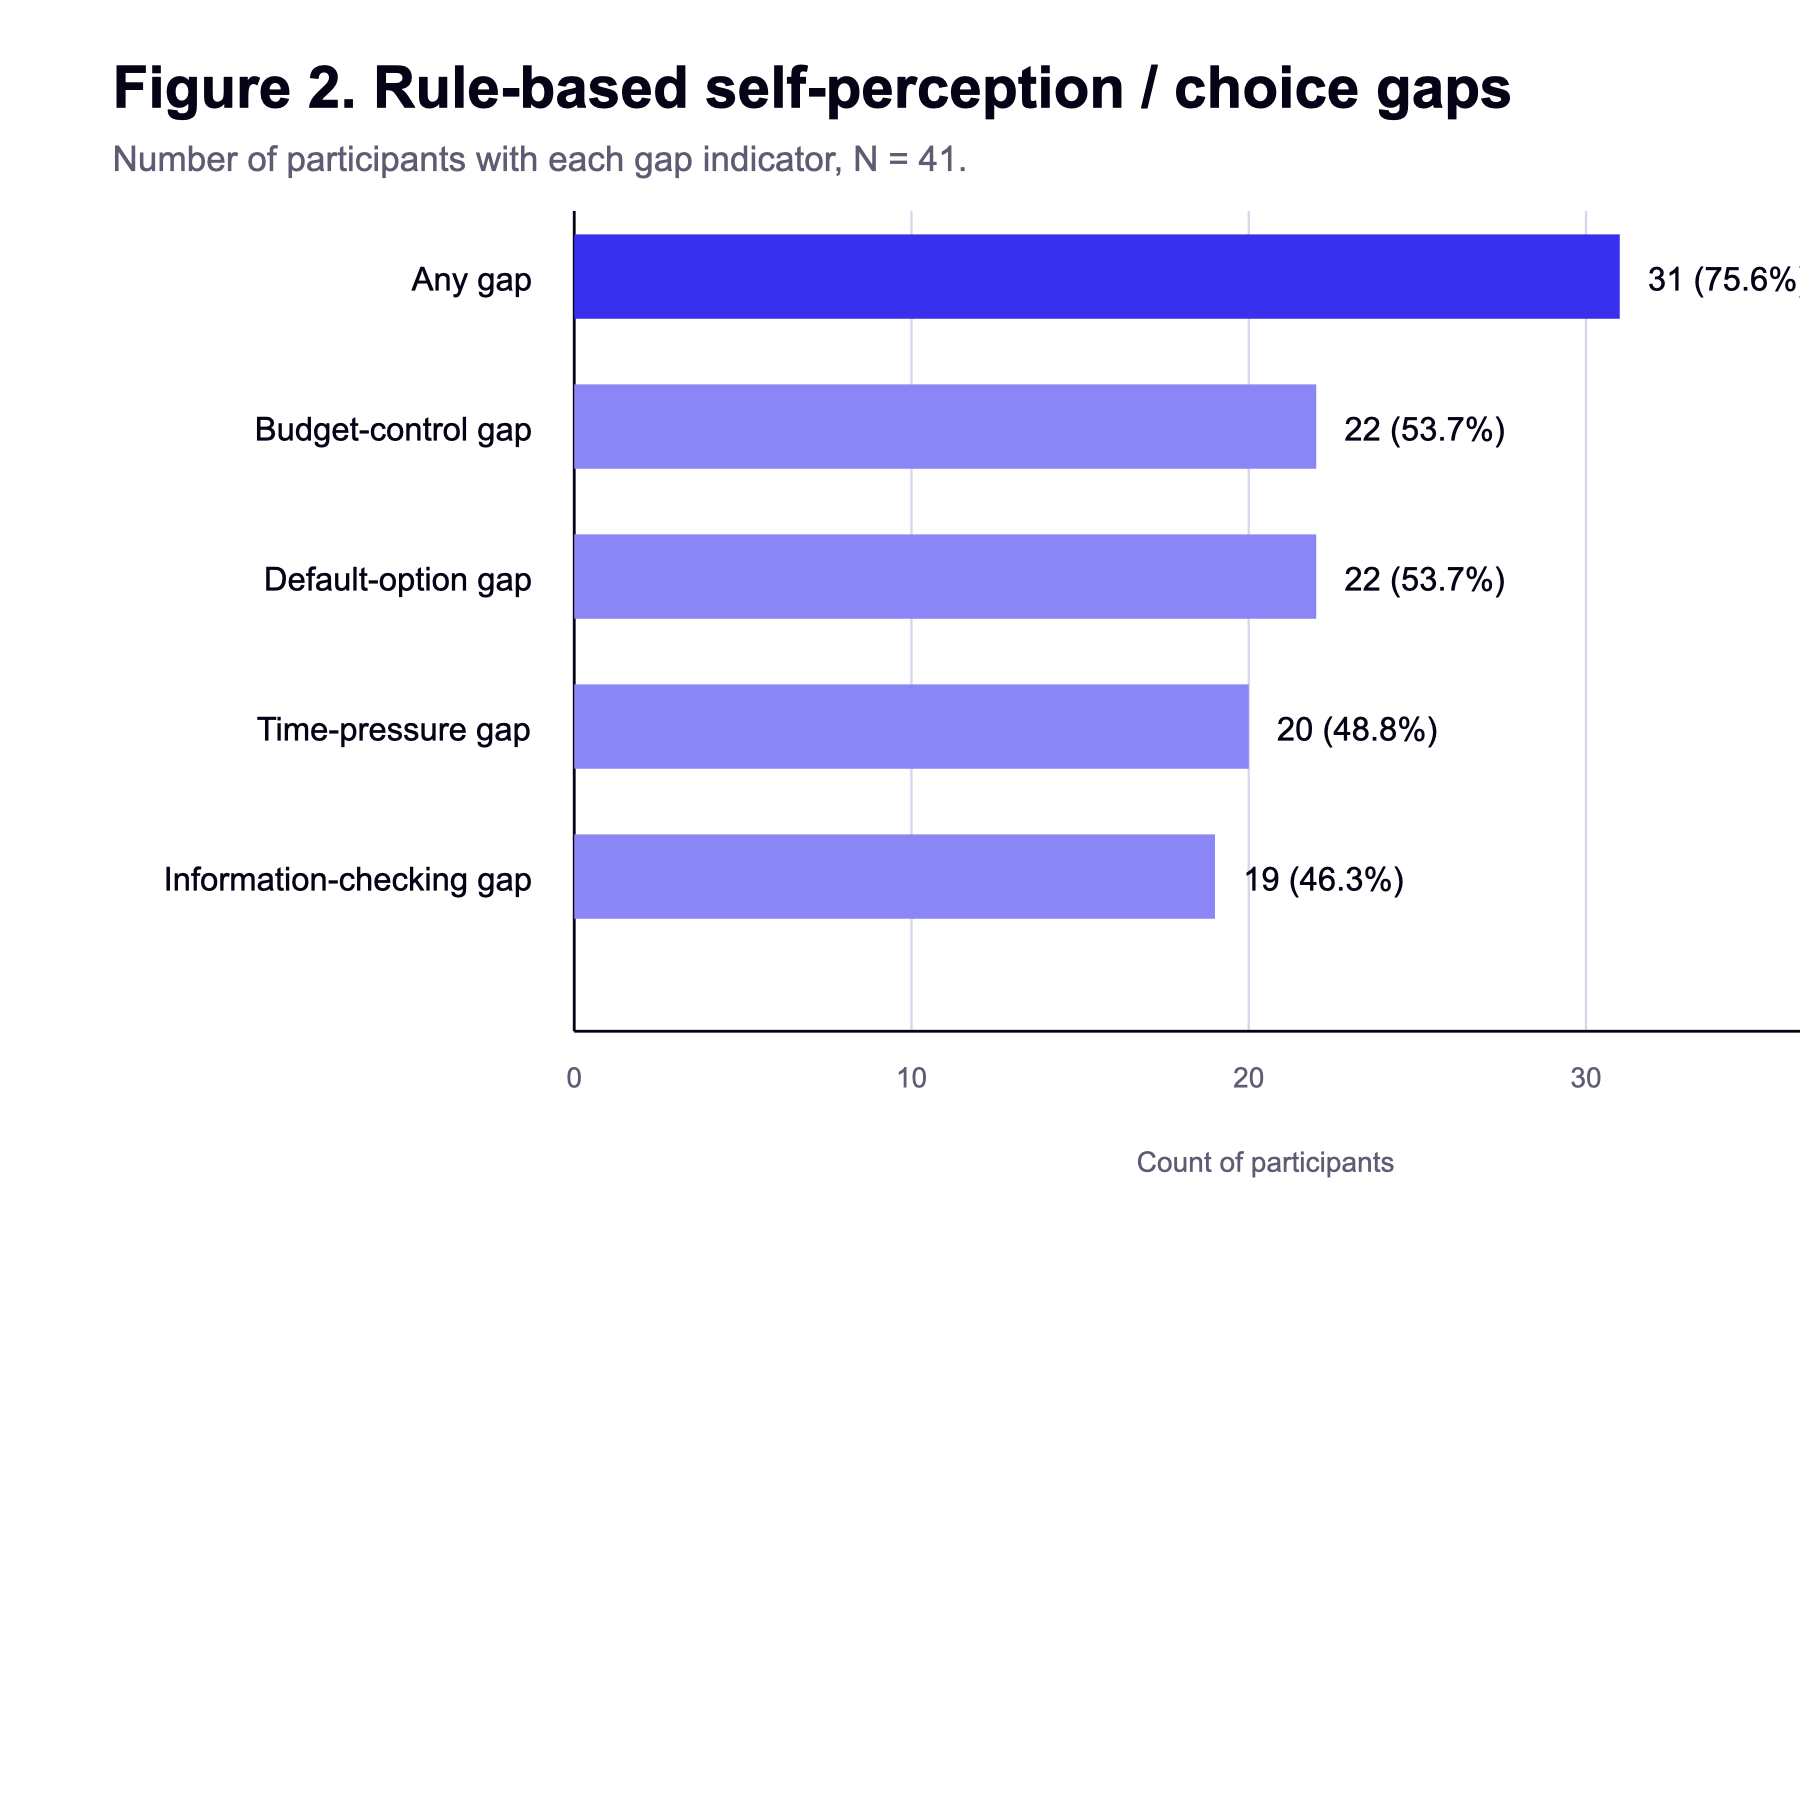
\includegraphics[width=.82\linewidth]{analysis/charts_png/gap-indicators.png}
  \caption{Rule-based self-perception and choice gaps.}
  \label{fig:gaps}
\end{figure}

\begin{figure}[H]
  \centering
  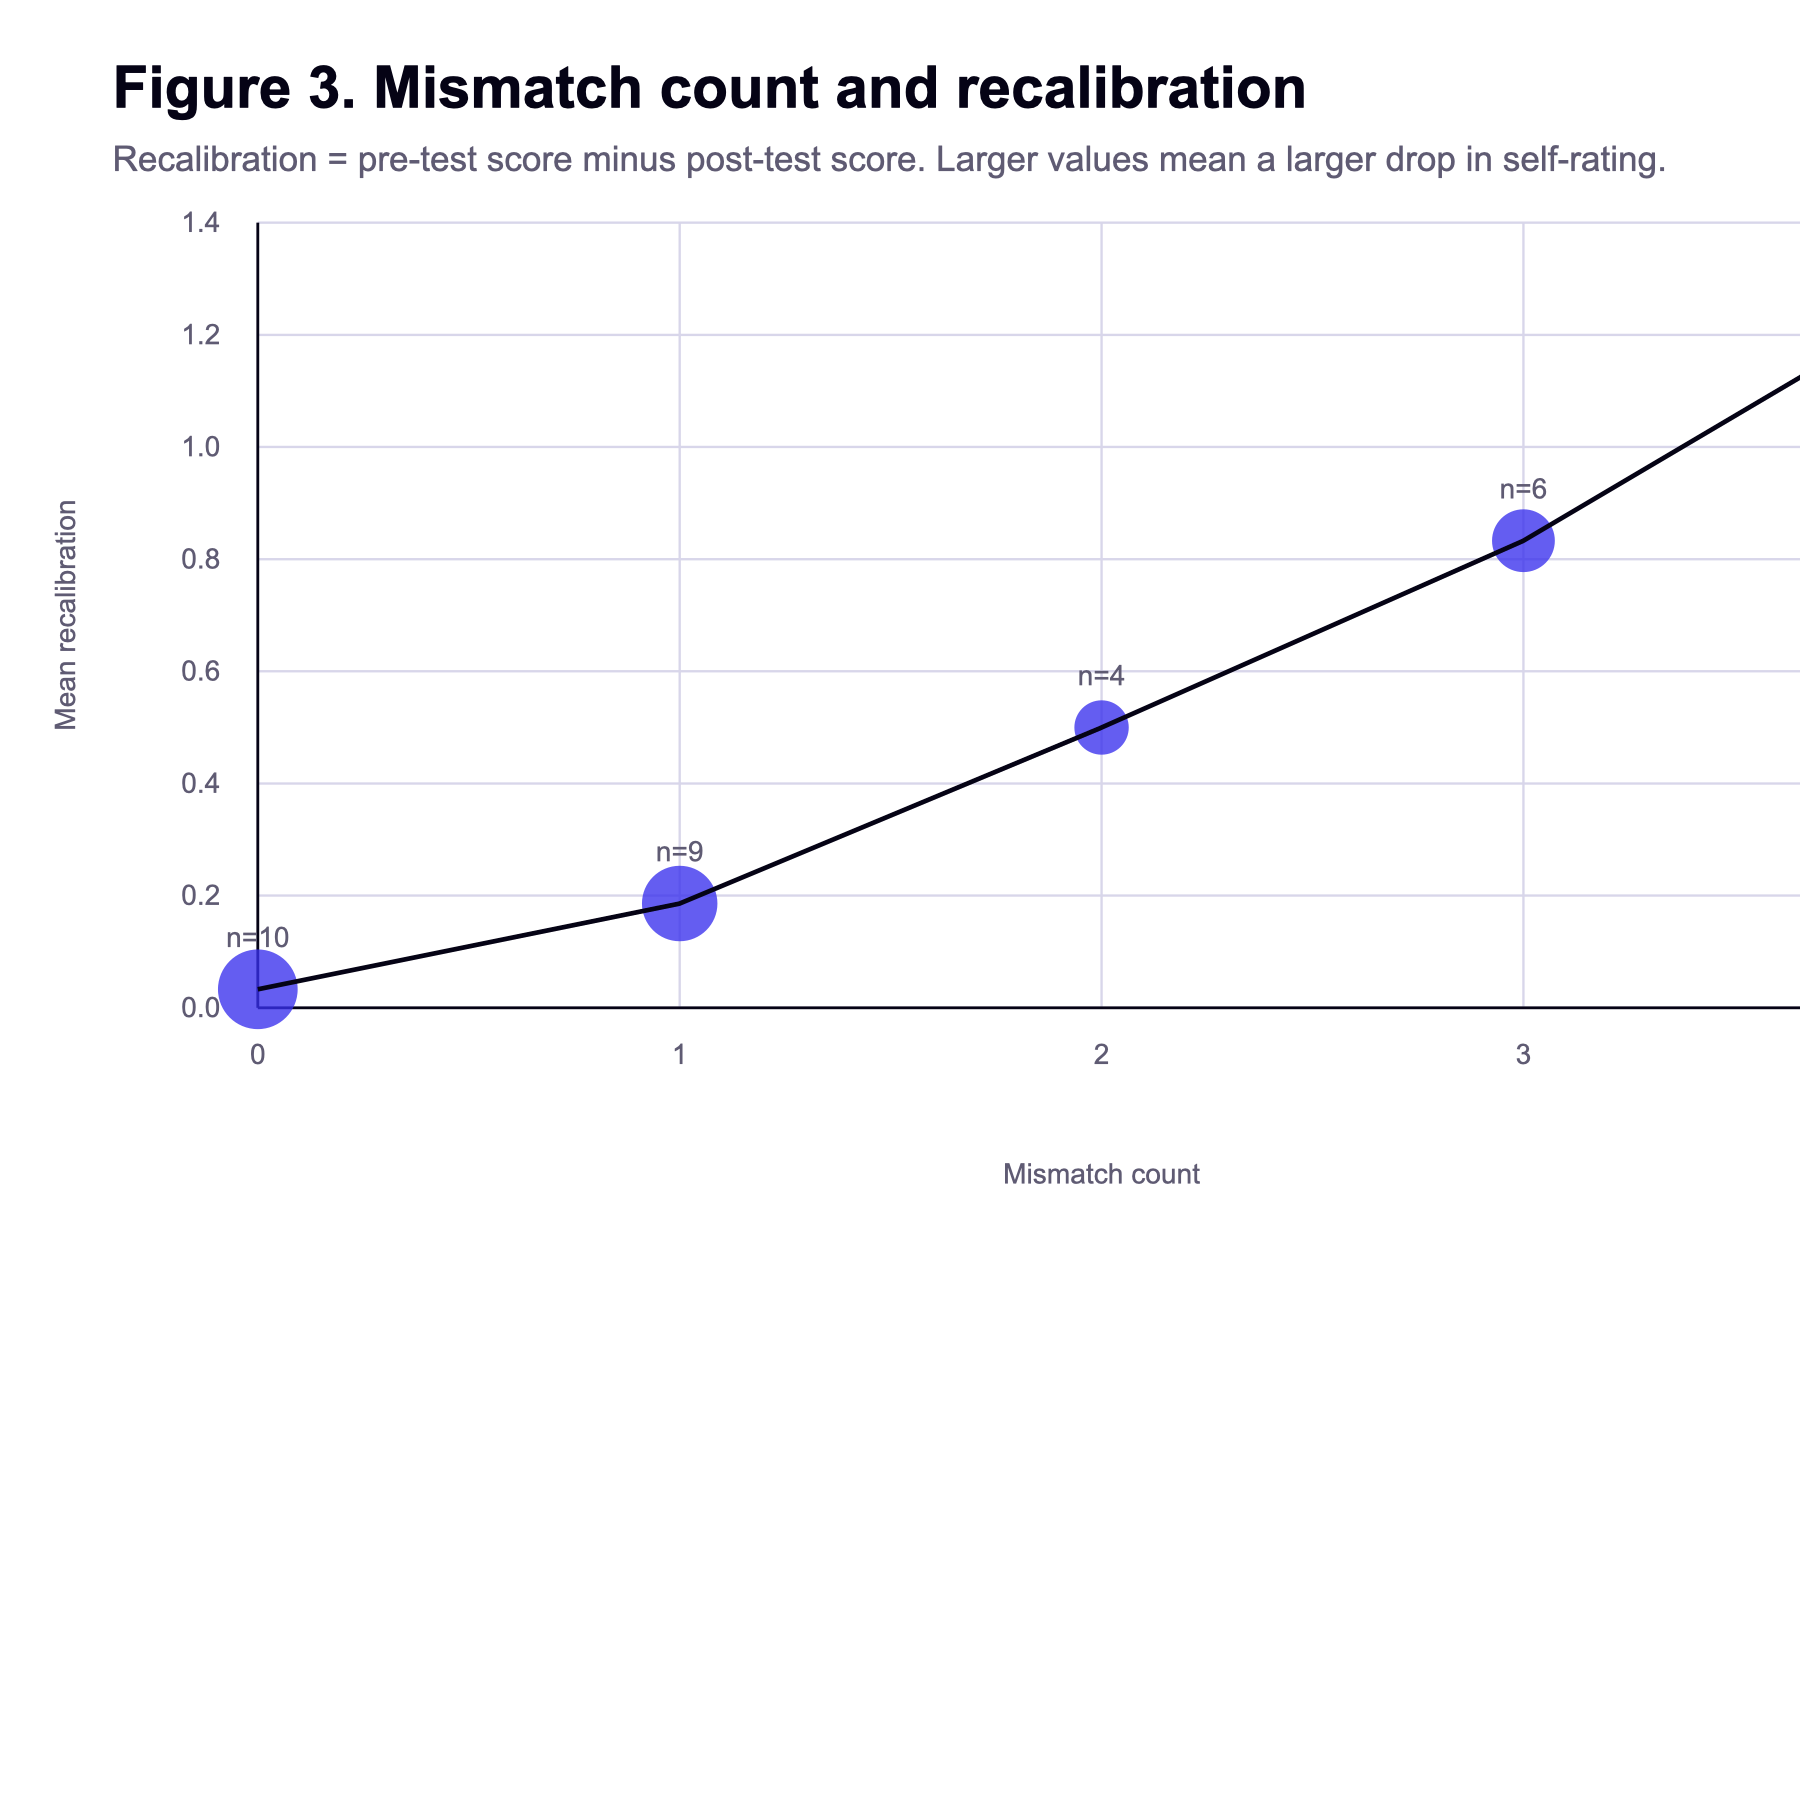
\includegraphics[width=.82\linewidth]{analysis/charts_png/mismatch-recalibration.png}
  \caption{Mismatch count and recalibration.}
  \label{fig:recalibration}
\end{figure}

\subsection{Open-Text Feedback}

The open-text feedback generally matched the quantitative pattern. Time pressure, discount reminders, or pop-ups appeared in 18 responses. Default service, checkout design, or add-on-related comments appeared in 20 responses. Information checking, reviews, rules, or unclear details appeared in 21 responses. Budget or price concern appeared in 10 responses. Product interest appeared in 11 responses, and direct self-recalibration language appeared in 14 responses.

Some participants directly described the gap between self-image and action, for example saying that they originally thought they would check reviews or control the budget, but acted more quickly in the simulated page.

Three representative anonymous responses illustrate this pattern. Translated from the original Chinese responses, one participant wrote, ``I thought I knew this kind of promotion trick, but I still clicked it.'' Another wrote, ``I thought I would compare more, but after seeing the price drop I quickly moved into checkout.'' A third wrote, ``I was very confident in my own judgment, but after adding something to the cart, I was more likely to continue along the process.''

\section{Discussion}

The results support the central idea of the project: high school students' consumer self-perception does not always match their simulated shopping choices. The strongest evidence is not only the pre/post score change, but the combination of three patterns. First, most participants showed at least one rule-based mismatch. Second, checkout default options and final submission under budget or review pressure produced high continuation rates. Third, participants with more mismatch indicators showed larger decreases in post-test self-rating.

The most important finding is the meaning of the lower post-test score. The original plan expected awareness to increase after the simulation. The actual result showed a decrease in self-rated ability to predict or explain one's own choices. This should be interpreted as a useful correction rather than a failure. Many participants may have entered the task with high confidence in their consumer judgment. After seeing their own simulated choices and the result comparison, they became less certain that their original self-image was accurate.

This interpretation keeps the original hypothesis visible instead of rewriting it after seeing the data. The expected direction was an increase in awareness, but the repeated items measured participants' confidence in their ability to predict or explain their own choices. A lower post-test score can therefore be read as a more cautious self-assessment. In other words, participants may have become more aware of the gap precisely because they no longer rated their own consumer judgment as highly as before.

The mismatch indicators strengthen this interpretation. The score decrease was not isolated from the behavioral data. Participants who showed more gaps between self-perception and simulated choice tended to show larger decreases in post-test self-rating. This pattern suggests that the artifact did not simply ask students whether they were careful consumers; it gave them a concrete record against which they could reconsider that self-description.

This interpretation connects with the literature on advertising literacy and self-report bias. Knowing how one wants to behave, or reporting that one is careful, does not guarantee that the same judgment will appear during a concrete choice. The simulation made this gap observable in a low-risk environment.

The project also shows why interface design matters. The default paid service was retained by 65.9\% of participants, and 70.7\% submitted the simulated order at the final stage. These patterns suggest that small page mechanisms may matter even when users have already described themselves as careful or information-aware consumers.

The open-text responses support the same interpretation. Participants did not only say that the website was interesting or confusing. Several responses named the exact page elements that shaped their decisions, such as the price-drop reminder, the default service, review conflict, or a product category they already liked. This matters because it links the quantitative pattern to the participant's own reflection. The simulation did not simply produce a score; it gave participants a concrete moment to notice how their self-description compared with their choices.

The study also suggests that product interest should be treated as an important background condition. A participant may be more likely to move forward when the product category is already personally relevant. This does not weaken the project. It shows that consumer judgment is situated. Budget, information checking, interface pressure, and product interest may work together rather than appear as separate causes.

The study has several limitations. First, the sample was small and came from a limited classroom context, so the findings should be treated as early evidence. Second, the artifact used a structured classroom simulation rather than a real commercial shopping app, so the analysis focuses on the shopping stages designed for this study. Third, the pre-test and post-test scores were still self-reported, so they measure participants' self-understanding, not an objective psychological state. Fourth, the mismatch indicators were rule-based and exploratory. They are useful for describing patterns, but they should be refined in future versions.

Another limitation concerns ecological realism. The artifact used a simplified shopping interface so that the study could record comparable actions across participants. This made the analysis cleaner, but it also reduced the complexity of real shopping platforms. Real platforms include longer browsing histories, stronger personalization, delivery timing, peer recommendations, payment friction, and repeated visits across time. The present simulation cannot capture all of those forces. It should be read as a controlled prototype that makes several common mechanisms visible.

The time data should also be interpreted carefully. Decision-time fields can show hesitation or fast movement through a stage, but they do not directly reveal why a participant hesitated. A longer time could mean careful checking, distraction, confusion, or technical delay. Future versions should combine timing with more precise interaction logs, such as scrolling, opening and closing the same page twice, or returning to a previous decision point.

Future work should improve the measurement design in three ways. The self-perception scale should be tested for clarity and reduced leading language. The shopping stages could add finer-grained micro-interaction records, such as scroll depth, repeated visits to the same element, and hesitation before final confirmation, if a more process-level analysis is needed. The result label should also be revised through participant feedback, so it describes behavior clearly without overclaiming personality diagnosis.

Future research could also compare two versions of the artifact. One version could include stronger shopping-interface cues, such as a more salient countdown or a default service. Another version could reduce those cues. Comparing the two versions would make it easier to separate general self-perception recalibration from the effect of specific interface mechanisms. A larger sample would also allow the analysis to compare product-interest groups, budget ranges, and different self-perception profiles more carefully.

Overall, the artifact appears useful as a classroom research tool. It does not prove that one interface causes a fixed consumer personality. It shows that a short shopping-platform simulation can help reveal where students' consumer self-image and simulated choices diverge.

\section{Conclusion}

This study examined whether an interactive shopping-platform simulation could reveal the gap between high school students' consumer self-perception and their simulated shopping choices. The results suggest that many participants entered the task with relatively high confidence in their ability to predict or explain their consumer behavior, but became more cautious after seeing their own choices in the simulation. The post-test score decreased on average, and this decrease was strongest among participants who showed more rule-based mismatches between what they said about themselves and what they clicked.

The main contribution of this project is the artifact itself. Instead of only asking students whether they are careful consumers, the website places them inside a controlled shopping-like environment and records concrete choices. This makes self-perception easier to compare with behavior. The study therefore suggests that a small interactive tool can support consumer education by helping students notice how interface cues, product interest, defaults, and time pressure may shape their choices.

The findings should be interpreted as early classroom evidence rather than a final causal claim. The sample was limited, the shopping environment was simulated, and the mismatch rules need further refinement. Even with these limits, the project shows a clear direction for future work: improving the measurement scale, testing different interface versions, and collecting more precise interaction data could make the tool more useful for studying how young consumers understand themselves in digital shopping environments.

\section{AI Disclosure}

The author used an AI assistant to convert the manuscript from Markdown into APA 7 LaTeX and to help check formatting and compilation issues. All research content, data, analysis, and references were reviewed by the author.


\section{References}
\begin{hangparas}{.25in}{1}
Atzmüller, C., \& Steiner, P. M. (2010). Experimental vignette studies in survey research. \textit{Methodology, 6}(3), 128--138. https://doi.org/10.1027/1614-2241/a000014

De Jans, S., Hudders, L., \& Cauberghe, V. (2018). Adolescents' self-reported level of dispositional advertising literacy: How do adolescents resist advertising in the current commercial media environment? \textit{Young Consumers, 19}(4), 402--420. https://doi.org/10.1108/YC-02-2018-00782

Donaldson, S. I., \& Grant-Vallone, E. J. (2002). Understanding self-report bias in organizational behavior research. \textit{Journal of Business and Psychology, 17}, 245--260. https://doi.org/10.1023/A:1019637632584

Friestad, M., \& Wright, P. (1994). The Persuasion Knowledge Model: How people cope with persuasion attempts. \textit{Journal of Consumer Research, 21}(1), 1--31. https://doi.org/10.1086/209380

John, D. R. (1999). Consumer socialization of children: A retrospective look at twenty-five years of research. \textit{Journal of Consumer Research, 26}(3), 183--213. https://doi.org/10.1086/209559

Mathur, A., Acar, G., Friedman, M. J., Lucherini, E., Mayer, J., Chetty, M., \& Narayanan, A. (2019). Dark patterns at scale: Findings from a crawl of 11K shopping websites. \textit{Proceedings of the ACM on Human-Computer Interaction, 3}(CSCW), Article 81. https://doi.org/10.1145/3359183

Nisbett, R. E., \& Wilson, T. D. (1977). Telling more than we can know: Verbal reports on mental processes. \textit{Psychological Review, 84}(3), 231--259. https://doi.org/10.1037/0033-295X.84.3.231

Rozendaal, E., Lapierre, M. A., van Reijmersdal, E. A., \& Buijzen, M. (2011). Reconsidering advertising literacy as a defense against advertising effects. \textit{Media Psychology, 14}(4), 333--354. https://doi.org/10.1080/15213269.2011.620540

Sproles, G. B., \& Kendall, E. L. (1986). A methodology for profiling consumers' decision-making styles. \textit{Journal of Consumer Affairs, 20}(2), 267--279. https://doi.org/10.1111/j.1745-6606.1986.tb00382.x

Steiner, P. M., Atzmüller, C., \& Su, D. (2017). Designing valid and reliable vignette experiments for survey research: A case study on the fair gender income gap. \textit{Journal of Methods and Measurement in the Social Sciences, 7}(2), 52--94. https://doi.org/10.2458/v7i2.20321
\end{hangparas}

\end{document}
